\documentclass{article}
\usepackage{titling}
\usepackage{lipsum}
\usepackage{amsmath}
\usepackage{listings}
\usepackage{graphicx}
\usepackage{subcaption}
\usepackage{pgfplots}
\usepgfplotslibrary{statistics}



\begin{document}
\noindent
\begin{minipage}[t]{0.6\textwidth}
    \begin{flushleft}
        \LARGE\textbf{Math 343 - Lab 3} \\
        \vspace{6pt} % add 6pt of vertical space
        \hrule width 10cm
        \vspace{12pt}
        \large\textbf{Preston Duffield} \\
        \large Western Washington University \\
        % \today
        April 18, 2023
        \vspace{24pt}
    \end{flushleft}
\end{minipage}

\section*{a)}
The hypothesis for the test is: \\
$H_0$: $\mu_1 = \mu_2 = \mu_3$. \\
$H_a$: At least one $\mu_i$ is different. \\
The test statistic $F = 7.91$. \\
The P-value = 0.006. \\
Since the P-value$< \alpha = 0.5$ we can conclude the following:
There is not enough statistic evidence to support the hypothesis that
$\mu_1 = \mu_2 = \mu_3$.

\section*{b)}
An estimate of the overall mean $\mu$, is given by the following:
\begin{align*}
    \hat{\mu} &= \frac{1}{a} \sum_{i=1}^{a} \hat{\mu_i} \\
              &= (13.4 + 38.2 + 73) / 4 \\
              &= 41.5\bar{3} \\
\end{align*}
An estimate of the variance $\sigma^2$ of the random error term
$\epsilon_{ij}$ can be pulled from the pooled standard deviation in Minitab:
\begin{align*}
    S_p ^2 &= 23.7978^2 = 566.335
\end{align*}

\clearpage
\section*{c)}
\begin{figure}[h]
    \centering
    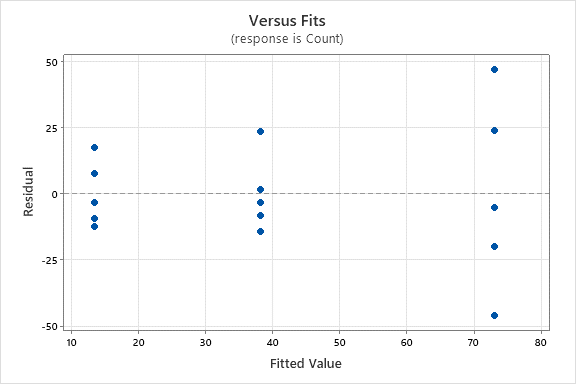
\includegraphics[width=1\textwidth]{./images/c.png}
    \caption{The residual plot from Minitab.}
    \label{fig:c}
  \end{figure}
The residual plot seems to indicate heteroskedasticity.
The data appears to have a bell like shape where data with a lower fitted value has a
smaller residual spread.
\clearpage
\section*{d)}
\begin{figure}[h]
    \centering
    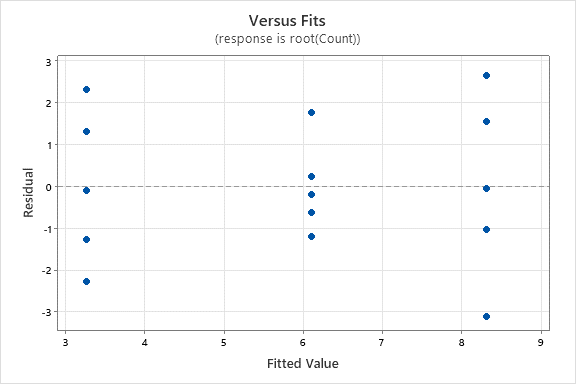
\includegraphics[width=1\textwidth]{./images/d.png}
    \caption{The residual plot from Minitab after a transformation on the response.}
    \label{fig:d}
  \end{figure}
It would seem that a transformation of a square root on the response has remedied the heteroskedasticity.
However more test should be performed to verify there are no more violations to the model assumptions. 
\section*{e)}


The hypothesis for the normality of the residuals is: \\
$H_0$: The data are drawn from a normal distribution. \\
$H_a$: The data are not drawn from a normal distribution.\\
The P-value = 0.801 for the Anderson-Darling normality test.
Since this P-value is larger than $\alpha$, we can conclude the following. \\
The evidence from the data is consistant with the data being drawn from a normal distribution.

\clearpage
\section*{f)}
The hypothesis for the Levene test for equality of population variances at $\alpha = 0.05$ is: \\
$H_0$: $\sigma_1^2 = \sigma_2^2 = \sigma_3^2$ \\
$H_a$: At least one $\sigma_i^2$ is different.\\

Since the P-value = 0.372 is greater than $\alpha = 0.05$, we can conclude the following.
The evidence from the data is consistant with $\sigma_1^2 = \sigma_2^2 = \sigma_3^2$,
ie, all of the variances are equal.

\section*{g)}
The hypothesis for the the Bartlett's test for equality of three population variances is the same as above.
Note that this test makes the strong assumtion that the data is distributed normally, and is only accurate if that assumption is met.
\subsection*{i.}
Since the P-value = 0.449 is greater than $\alpha$, this test results in the same conclusion as above.
That is, the evidence from the data is consistant with all of the variances being equal.
\subsection*{ii.}
If there were a considerable difference in the results from the 2 tests I would check the following:
\begin{enumerate}
    \item Check if the data is normal through a hypothesis test.
    \item If the data was normal, I would trust the Bartletss test for the following reasons:
    \begin{itemize}
        \item This test assumes normallity and the data is normally distributed.
        \item This test is more powerful than Levenes.
    \end{itemize}
    \item If the data was \textbf{not} normal, I would trust the Modified Levenes test for the following reasons:
    \begin{itemize}
        \item This test is robust for normaility.
    \end{itemize}
\end{enumerate}

\clearpage
\section*{h)}

The predicted value of the after-treatment particle count for the $1^{st}$ method is $3.26252^2 = 10.64$.


\end{document}